\section{Manipulation Methods}
\label{sec:manipulation_methods}

As outlined in \autoref{sec:interpretation_methods}, there are a variety of explanation methods readily available as frameworks and open source implementations. However, there is still little analysis on the robustness and reliability of such methods. 
While it is already common practice to test machine learning models against adversarial attacks, the same is not yet the standard for interpretation methods. We argue that these techniques should not be used in critical applications without basic testing of interpretation techniques against adversarial settings.

\subsection{Adversarial Setting}
\label{}




The focus of most works is on adversarial attacks against the prediction of a machine learning model. Contrary, the focus of this paper is on the attacks on the interpretation without changing the prediction.

A manipulation method refers to a method influencing an interpretation method $\mathcal{I}$ to yield a wrong interpretation. This influence on the interpretation method is also called \textit{fooling} or an \textit{attack}. 

The goal is to apply efficient and for humans imperceptible perturbations to change the interpretability of the input sample while leaving the prediction unchanged. 

Formally, the problem can be defined as: 
\textbf{Definition 2: Interpretation Manipulation Method}\\
% as it is the goal to disclose the vulnerability of the explanation method and not the vulnerability of the model.
A manipulation method $\mathcal{F}$ is defined as a method for altering the output of an explanation method while leaving the model performance of the neural network $N$ roughly unchanged. 
This must be the case, as the attack is targeted to fool the explanation method, and is essentially not targeted to fool the model itself. Fooling the model would only disclose the vulnerability of the model but would not allow to gain insight into the stability of the fooling method. 
Hence, the main criteria for an explanation manipulation method must be fulfilled: 
\begin{enumerate}
    \item[1.] The models prediction stays approximately the same, i.e. $f_N(x_{adv}) \approx f_N(x)$ or $f_{N_{adv}}(x) \approx f_N(x)$
    \item[2.] The explanation map $h(x_{adv})$ is significantly different to the explanation map resulting from non adversarial models or inputs $h(x)$, i.e. $h(x_{adv})$ or $$\argmax_{\delta} = \mathcal{D}(\mathcal{I}(x_i, \boldsymbol{\omega}), \mathcal{I}(x_i+\delta, \boldsymbol{\omega})$$
    \item[3.] In case the attack is in the input domain of the model, the perturbation of input samples must be imperceptible by humans. According to \cite{dombrowski2019explanations}, the norm of the added perturbation $\delta$ to an input sample $x$ thus must be small, i.e. $\norm{\delta x} = \norm{x_{adx}-x}_{\inf} \leq \epsilon$ % https://arxiv.org/pdf/1710.10547.pdf 
\end{enumerate}

Other criteria to a manipulation method are the following:

\noindent\textbf{Effectiveness.} The manipulation scheme is inexpensive to conduct. Input manipulations are by definition inexpensive, as the perturbation can be applied to single input samples. Model manipulations are more expensive as they require tho model parameters to be adapted. However, an adversarial model can be obtained by fine-tuning the model with an adapted objective function. This fine-tuning also has the advantage that the model is adapted to include a systematic bias and can thus be applied to fool explanation methods without further adapting the model or input samples.

\noindent\textbf{Transferability.} The manipulation does not only fool one type of explanation method, but it's effect transfers to other types. 



Most of the explanation methods outlined in sec. \autoref{sec:interpretation_methods} have been shown to be vulnerable to adversarial perturbations. 
Manipulation methods often show that there exist small feature changes resulting in a change of the explanation methods output while the output of the model itself does not change. 
Most approaches aim at providing a relevance measure of the input features. \\



%%%%%%%%%%
\subsection{Manipulation Levels}
\label{subsec:manipulation_levels}

\noindent\textbf{Adversarial Input Manipulation.} The general approach is to perturb input data while observing the effect of this perturbation on the model prediction. As found in TODO, visually-imperceptible perturbations of an input image can make explanations worse for the same model and interpreter. 

\begin{figure}[t]
    \centering
    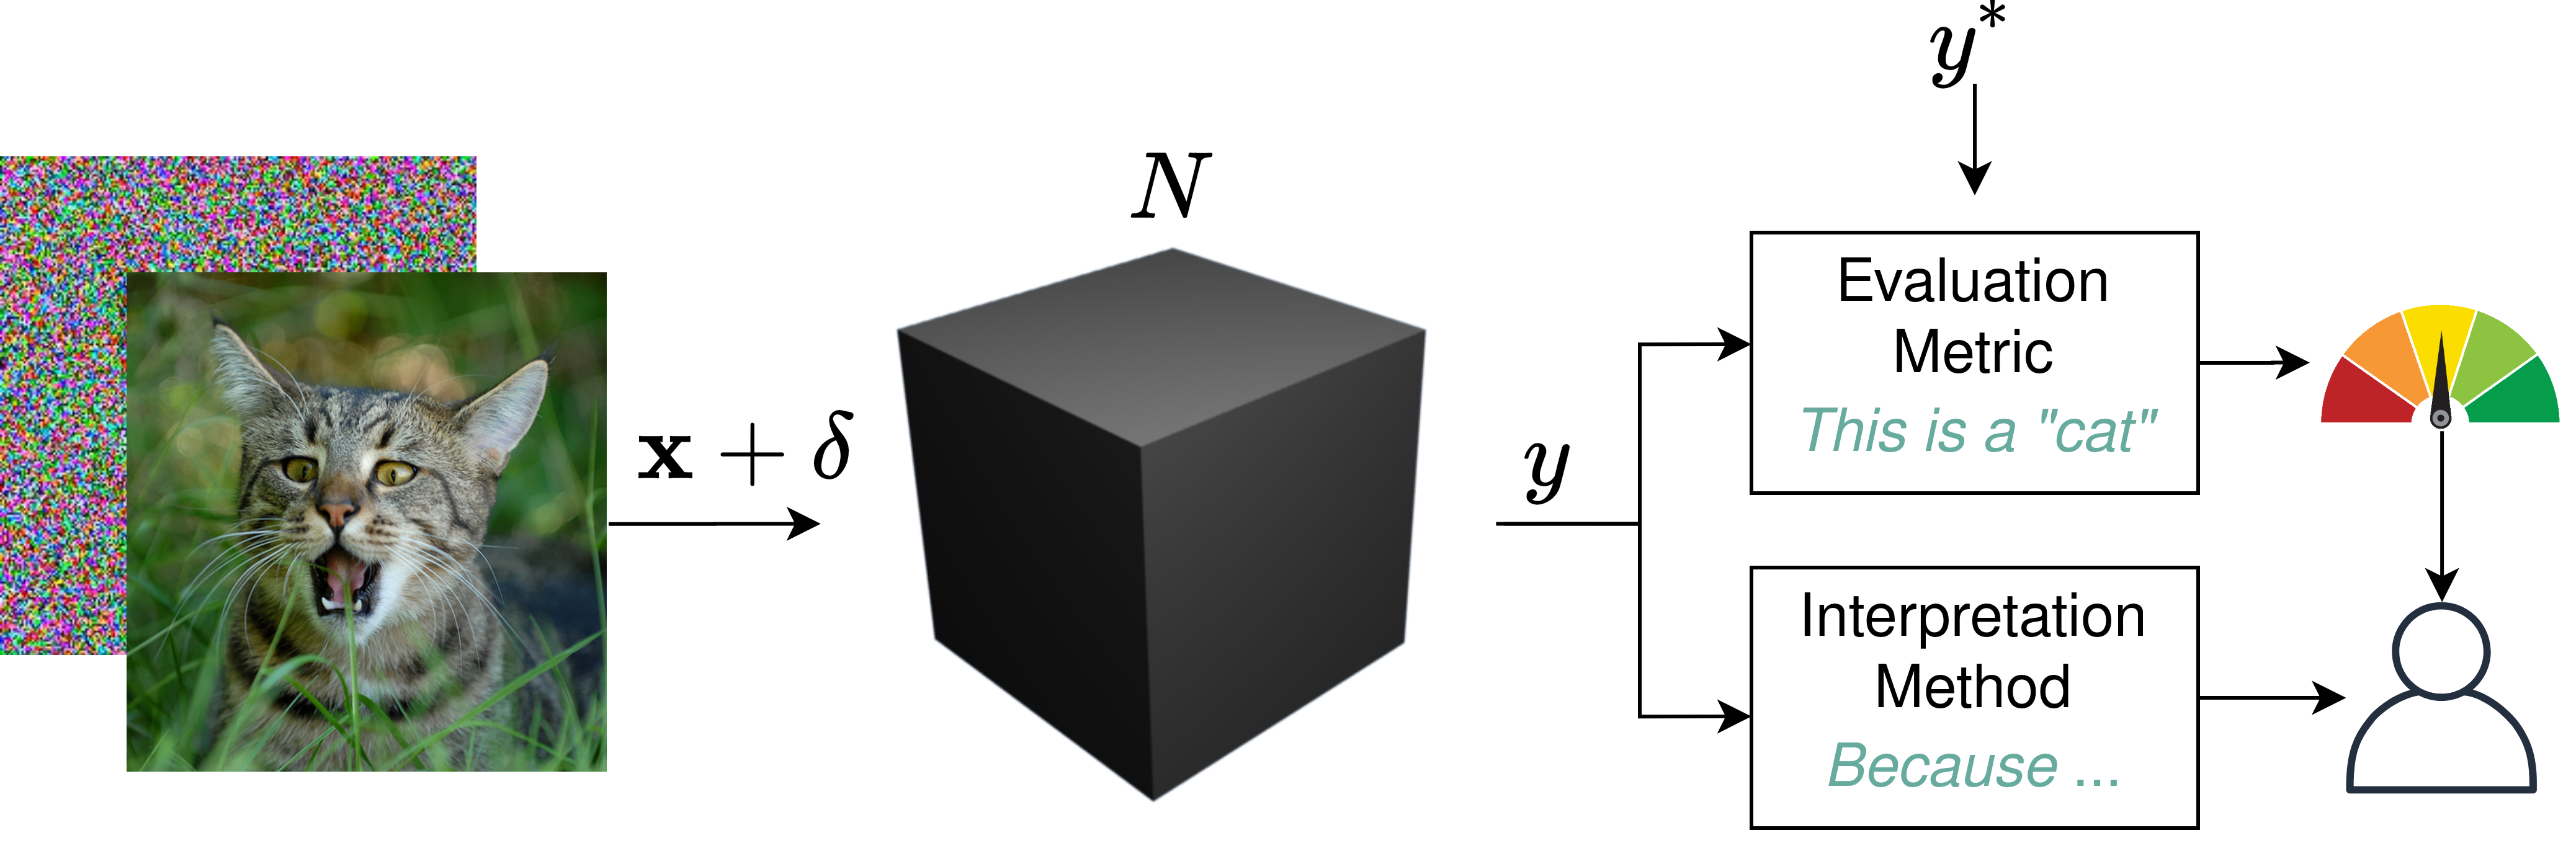
\includegraphics[width=\linewidth]{figures/input_manipulations.png}
    \caption{Depiction of an adversarial input manipulation. The model is fine-tuned with altered input samples.}
    \label{fig:input_manipulation}
    \vspace{-0.3cm}
\end{figure}

\noindent\textbf{Adversarial Model Manipulation.} 
Contrary to input manipulations, model manipulations do not operate on the input space but rather on the model parameter space itself. 
As first introduced by Heo et al. \cite{fooling_nn_interpreters} in 2017, this line of research is comparably new. 
Adversarial model manipulations are obtained by fine-tuning the model on the same data but with an adapted objective function. \cite{fooling_nn_interpreters} propose the adapted loss function of $$ \mathcal{L} = \mathcal{L}_{CE}(\mathcal{D};\omega) + \lambda \cdot \mathcal{L}(\mathcal{D};\omega; \omega_0) $$ where $\mathcal{L}_{CE}$ would be the standard cross-entropy classification loss. 

\begin{figure}[t]
    \centering
    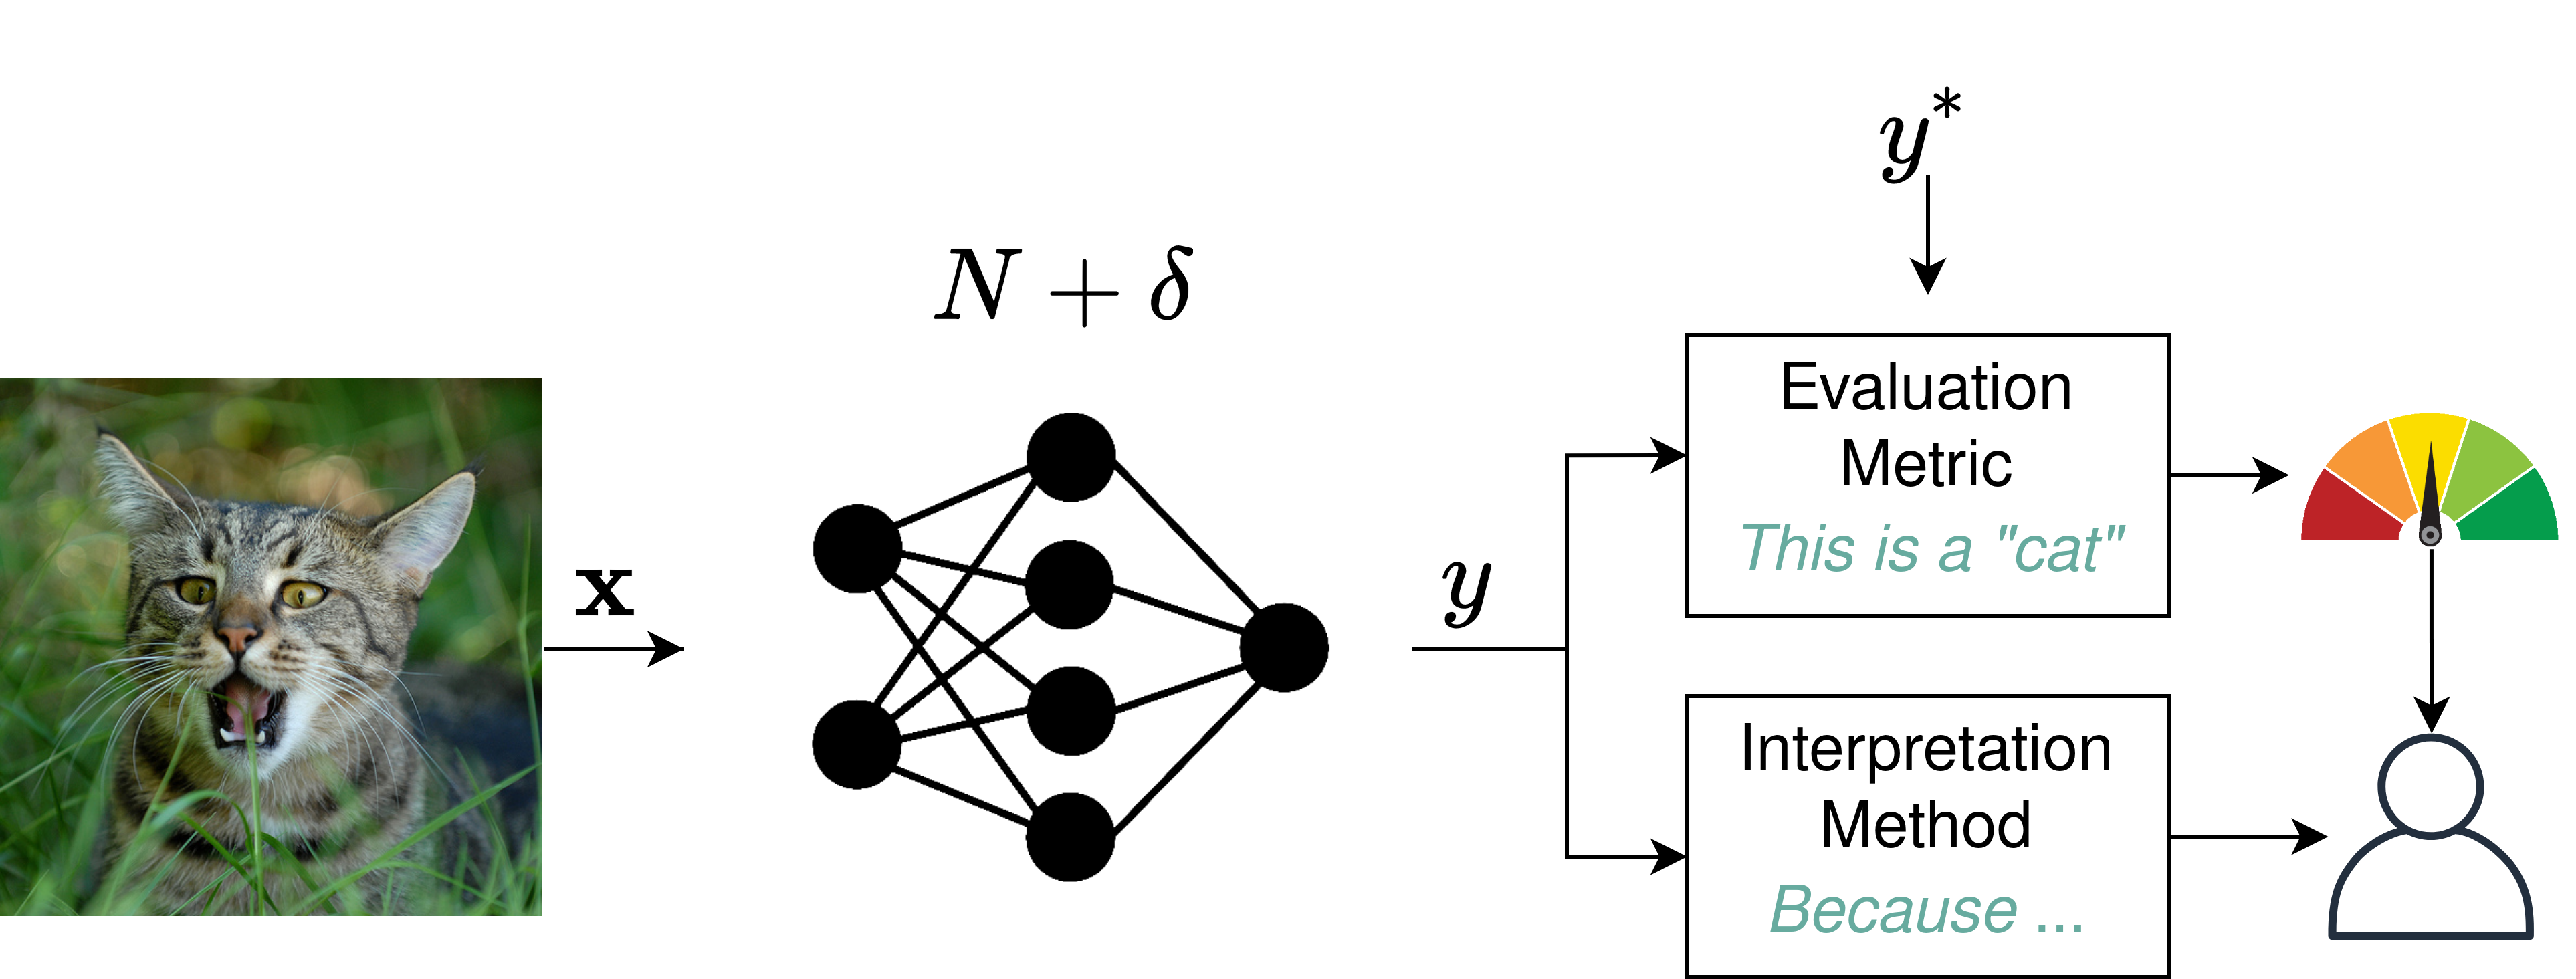
\includegraphics[width=\linewidth]{figures/model_manipulations.png}
    \caption{Depiction of an adversarial model manipulation. The model is fine-tuned with the same distribution of input data and a fooling loss.}
    \label{fig:input_manipulation}
    \vspace{-0.3cm}
\end{figure}

The authors find that perturbed model parameters can also make explanations worse for the same input images and interpreters. 

Creation of a fooled model by fine-tuning the model with a fooling loss. 
% https://github.com/rmrisforbidden/Fooling_Neural_Network-Interpretations/blob/master/Materials/PPT.pdf 



\subsubsection{Transferability of Manipulations}
\cite{fooling_nn_interpreters} find that fooling one explanation method with a fooling scheme transfers to other methods. 


%%%%%%%%%%
\subsection{Manipulation Targets}
\label{subsec:manipulation_targets}
In addition to the categorization of manipulation methods based on the manipulation level, the methods can further be categorized based on the target of their perturbation. The first possibility is untargeted perturbation. The second is targeted perturbation. Both these styles can be applied on either model and input level. 

\noindent\textbf{Untargeted Manipulations.} 
The majority of manipulations is untargeted, meaning that the applied perturbations are mostly random and not designed to change the prediction for a specific portion of an input sample. 

\noindent\textbf{Targeted Manipulations.} 
On the contrary, targeted manipulations are designed to specificly alter the explanation of distinct features of an input instance. Such a specific feature might be an object in the input image in the context of image classification. 
For instance \cite{fooling_nn_interpreters} introduce a fooling scheme in which the interpretations of the classes elephant and school bus are swapped. 
Manipulations on the level of the model are mostly targeted, as the explanation methods are being fooled by adapting the model parameters. 

% Model manipulations pose a much higher threat for deploying the models: If a model itself is changed to explicitly, systemactically fool an explanation method, the bias of the model is internal and much harder to reveal than just a different sort of input into the model. 



\subsection{Evaluation Criteria}
\label{subsec:evaluation_criteria}
As outlined in section \autoref{sec:manipulation_methods}, there exists a plethora of interpretations methods differing in the assumption about the model character and also in style how interpretations are obtained. Thus, reliable evaluation methods are required allowing for a choice of an appropriate and robust explanation method. 
Evaluations of the quality of an explanation method can be separated into qualitative and quantitative evaluations. 
% \cite{fooling_nn_interpreters} propose to measure the quality of an explanation method by their stability with respect to adversarial model manipulations. 



\mypar{Quantitative Evaluations.} 
As the goal of interpreter manipulations is to fool an interpreter, thus altering the output of in interpreter, it is straightforward to compare interpretations before and after perturbation \cite{ghorbani2019interpretation}.
Common metrics for quantitatively measuring this similarity between interpretations are the following: 
\begin{itemize}
    \item \textbf{Spearman's rank order correlation.} As interpretation methods rank the features based on their importance, the rank correlation \cite{spearman1961proof} is a natural meusure for comparing interpretations. 
    \item \textbf{Intersection of the top-$k$ features.} For some tasks, only the top-$k$ features are relevant, such that a comparison between these top-$k$ features is insightful. 
    \item \textbf{Fooling Success Rate (FSR).} Heo et al. \cite{fooling_nn_interpreters} introduce the concept of the Fooling Success Rate (FSR) with the aim to create a measure for systematically measuring the robustness of an interpretation method to adversarial model manipulations. The FSR measures on how many samples from a dataset an interpretation method $\mathcal{I}$ is fooled by a model manipulation. The higher the FSR, the more often an inetpretation method is fooled. 
\end{itemize}


\mypar{Qualitative Evaluations.} 
As interpretations are attributed to input features, the resulting relevance values $l$ can be easily mapped to the input vector $x$.
Looking at these evaluations for specific samples is informative albeit not usable to obtain a general statistic about the explanation methods quality.
